\documentclass{report}

\usepackage{amsmath, amssymb}
\usepackage[]{graphicx}
\usepackage[]{color}
\usepackage{tikz}

\newcommand{\roundpic}[4][]{
  \tikz\node [circle, minimum width = #2,
    path picture = {
      \node [#1] at (path picture bounding box.center) {
        \includegraphics[width=#3]{#4}};
    }] {};}
    
%% commands from jss.cls
\newcommand\code{\bgroup\@makeother\_\@makeother\~\@makeother\$\@codex}
\def\@codex#1{{\normalfont\ttfamily\hyphenchar\font=-1 #1}\egroup}
% \let\code=\texttt
\let\proglang=\textsf
\newcommand{\pkg}[1]{{\fontseries{b}\selectfont #1}}
\newcommand{\email}[1]{\href{mailto:#1}{\normalfont\texttt{#1}}}
\newcommand{\E}{\mathsf{E}}
\newcommand{\VAR}{\mathsf{VAR}}
\newcommand{\COV}{\mathsf{COV}}
\newcommand{\Prob}{\mathsf{P}}

\usepackage{bm}
\newcommand{\bb}{\bm{\beta}}
\newcommand{\dif}{\mathrm{d}}
\newcommand{\bg}{\bm{\gamma}}
\newcommand{\bth}{\bm{\theta}}
\newcommand{\bx}{\bm{x}}
\newcommand{\ox}{\overline{x}}
\newcommand{\obx}{\overline{\bm{x}}}

%% maxwidth is the original width if it is less than linewidth
%% otherwise use linewidth (to make sure the graphics do not exceed the margin)
\makeatletter
\def\maxwidth{ %
  \ifdim\Gin@nat@width>\linewidth
    \linewidth
  \else
    \Gin@nat@width
  \fi
}
\makeatother

\definecolor{fgcolor}{rgb}{0.345, 0.345, 0.345}
\newcommand{\hlnum}[1]{\textcolor[rgb]{0.686,0.059,0.569}{#1}}%
\newcommand{\hlstr}[1]{\textcolor[rgb]{0.192,0.494,0.8}{#1}}%
\newcommand{\hlcom}[1]{\textcolor[rgb]{0.678,0.584,0.686}{\textit{#1}}}%
\newcommand{\hlopt}[1]{\textcolor[rgb]{0,0,0}{#1}}%
\newcommand{\hlstd}[1]{\textcolor[rgb]{0.345,0.345,0.345}{#1}}%
\newcommand{\hlkwa}[1]{\textcolor[rgb]{0.161,0.373,0.58}{\textbf{#1}}}%
\newcommand{\hlkwb}[1]{\textcolor[rgb]{0.69,0.353,0.396}{#1}}%
\newcommand{\hlkwc}[1]{\textcolor[rgb]{0.333,0.667,0.333}{#1}}%
\newcommand{\hlkwd}[1]{\textcolor[rgb]{0.737,0.353,0.396}{\textbf{#1}}}%
\let\hlipl\hlkwb

\usepackage{framed}
\makeatletter
\newenvironment{kframe}{%
 \def\at@end@of@kframe{}%
 \ifinner\ifhmode%
  \def\at@end@of@kframe{\end{minipage}}%
  \begin{minipage}{\columnwidth}%
 \fi\fi%
 \def\FrameCommand##1{\hskip\@totalleftmargin \hskip-\fboxsep
 \colorbox{shadecolor}{##1}\hskip-\fboxsep
     % There is no \\@totalrightmargin, so:
     \hskip-\linewidth \hskip-\@totalleftmargin \hskip\columnwidth}%
 \MakeFramed {\advance\hsize-\width
   \@totalleftmargin\z@ \linewidth\hsize
   \@setminipage}}%
 {\par\unskip\endMakeFramed%
 \at@end@of@kframe}
\makeatother

\definecolor{shadecolor}{rgb}{.97, .97, .97}
\definecolor{messagecolor}{rgb}{0, 0, 0}
\definecolor{warningcolor}{rgb}{1, 0, 1}
\definecolor{errorcolor}{rgb}{1, 0, 0}
\newenvironment{knitrout}{}{} % an empty environment to be redefined in TeX

% added for using R markdown
\usepackage{fancyvrb}
\newcommand{\VerbBar}{|}
\newcommand{\VERB}{\Verb[commandchars=\\\{\}]}
\DefineVerbatimEnvironment{Highlighting}{Verbatim}{commandchars=\\\{\}}
% Add ',fontsize=\small' for more characters per line
\usepackage{framed}
\definecolor{shadecolor}{RGB}{248,248,248}
\newenvironment{Shaded}{\begin{snugshade}}{\end{snugshade}}
\newcommand{\AlertTok}[1]{\textcolor[rgb]{0.94,0.16,0.16}{#1}}
\newcommand{\AnnotationTok}[1]{\textcolor[rgb]{0.56,0.35,0.01}{\textbf{\textit{#1}}}}
\newcommand{\AttributeTok}[1]{\textcolor[rgb]{0.77,0.63,0.00}{#1}}
\newcommand{\BaseNTok}[1]{\textcolor[rgb]{0.00,0.00,0.81}{#1}}
\newcommand{\BuiltInTok}[1]{#1}
\newcommand{\CharTok}[1]{\textcolor[rgb]{0.31,0.60,0.02}{#1}}
\newcommand{\CommentTok}[1]{\textcolor[rgb]{0.56,0.35,0.01}{\textit{#1}}}
\newcommand{\CommentVarTok}[1]{\textcolor[rgb]{0.56,0.35,0.01}{\textbf{\textit{#1}}}}
\newcommand{\ConstantTok}[1]{\textcolor[rgb]{0.00,0.00,0.00}{#1}}
\newcommand{\ControlFlowTok}[1]{\textcolor[rgb]{0.13,0.29,0.53}{\textbf{#1}}}
\newcommand{\DataTypeTok}[1]{\textcolor[rgb]{0.13,0.29,0.53}{#1}}
\newcommand{\DecValTok}[1]{\textcolor[rgb]{0.00,0.00,0.81}{#1}}
\newcommand{\DocumentationTok}[1]{\textcolor[rgb]{0.56,0.35,0.01}{\textbf{\textit{#1}}}}
\newcommand{\ErrorTok}[1]{\textcolor[rgb]{0.64,0.00,0.00}{\textbf{#1}}}
\newcommand{\ExtensionTok}[1]{#1}
\newcommand{\FloatTok}[1]{\textcolor[rgb]{0.00,0.00,0.81}{#1}}
\newcommand{\FunctionTok}[1]{\textcolor[rgb]{0.00,0.00,0.00}{#1}}
\newcommand{\ImportTok}[1]{#1}
\newcommand{\InformationTok}[1]{\textcolor[rgb]{0.56,0.35,0.01}{\textbf{\textit{#1}}}}
\newcommand{\KeywordTok}[1]{\textcolor[rgb]{0.13,0.29,0.53}{\textbf{#1}}}
\newcommand{\NormalTok}[1]{#1}
\newcommand{\OperatorTok}[1]{\textcolor[rgb]{0.81,0.36,0.00}{\textbf{#1}}}
\newcommand{\OtherTok}[1]{\textcolor[rgb]{0.56,0.35,0.01}{#1}}
\newcommand{\PreprocessorTok}[1]{\textcolor[rgb]{0.56,0.35,0.01}{\textit{#1}}}
\newcommand{\RegionMarkerTok}[1]{#1}
\newcommand{\SpecialCharTok}[1]{\textcolor[rgb]{0.00,0.00,0.00}{#1}}
\newcommand{\SpecialStringTok}[1]{\textcolor[rgb]{0.31,0.60,0.02}{#1}}
\newcommand{\StringTok}[1]{\textcolor[rgb]{0.31,0.60,0.02}{#1}}
\newcommand{\VariableTok}[1]{\textcolor[rgb]{0.00,0.00,0.00}{#1}}
\newcommand{\VerbatimStringTok}[1]{\textcolor[rgb]{0.31,0.60,0.02}{#1}}
\newcommand{\WarningTok}[1]{\textcolor[rgb]{0.56,0.35,0.01}{\textbf{\textit{#1}}}}

\usepackage{alltt}
\usepackage{graphicx}
\usepackage[margin=1cm]{geometry}
\usepackage{color}
\usepackage[pages=absolute]{flowfram}
\usepackage{lipsum}
\usepackage{url, pdfpages}
\usepackage{enumitem}
\setlist{itemsep = 0pt, topsep = 1pt, leftmargin = 0.6mm}
\usepackage[anythingbreaks]{breakurl}
\usepackage{microtype}
\usepackage{anyfontsize}
\usepackage{caption}
\usepackage{subcaption}
\renewcommand{\figurename}{Fig.}
\usepackage{wrapfig}
\usepackage{scrextend}
\usepackage{booktabs}

% added
\usepackage{natbib}

\renewcommand{\UrlBreaks}{\do\/\do\a\do\b\do\c\do\d\do\e\do\f\do\g\do\h\do\i\do\j\do\k\do\l\do\m\do\n\do\o\do\p\do\q\do\r\do\s\do\t\do\u\do\v\do\w\do\x\do\y\do\z\do\A\do\B\do\C\do\D\do\E\do\F\do\G\do\H\do\I\do\J\do\K\do\L\do\M\do\N\do\O\do\P\do\Q\do\R\do\S\do\T\do\U\do\V\do\W\do\X\do\Y\do\Z}

\usepackage{algorithm, algorithmic}

% added to make font size smaller in code output
\usepackage{etoolbox}
\AtBeginEnvironment{verbatim}{\vspace{-10pt}\begin{small}}
\AtEndEnvironment{verbatim}{\medskip\end{small}}
\renewenvironment{Shaded}{\begin{small}\begin{snugshade}}
{\end{snugshade}\end{small}}


%% for knitr
\usepackage[unicode=true,pdfusetitle,
 bookmarks=true,bookmarksnumbered=true,bookmarksopen=true,bookmarksopenlevel=2,
 breaklinks=false,pdfborder={0 0 1},backref=false,colorlinks=false]
 {hyperref}
\hypersetup{
 pdfstartview={XYZ null null 1}}

% graph path
\graphicspath{{images/}}
\DeclareGraphicsExtensions{.eps,. ps,. pdf, .jpg, .png}

\twocolumn

\begin{document}


% \section*{Software Review}
\section*{Recurrent Event Analysis with \proglang{R} packages \pkg{reda} and \pkg{reReg}}

Recurrent event data arise when the event of interest,
such as hospital admissions, infections, or tumor recurrences,
can recur in the same individual during follow-up.
The standard ``time-to-first'' event analysis cannot capture the cumulative experience of
the recurrent events and could lead to invalid inferences.
The \proglang{R} packages \pkg{reda} \citep{reda-package} and \pkg{reReg} \citep{reReg-package}
provide a collection of methods for exploring and analyzing 
recurrent event data.


Consider a random sample of $n$ subjects and let
$N_i(t)$ be the number of events the $i$th subject experienced over the interval $[0, t]$. 
Let $D$ be the failure time of interest that could either be a terminal event (e.g., death)
or a non-terminal event (e.g., treatment failure).
Let $C$ be the potential censoring time for reasons other than the failure event
(e.g., study dropouts).
The observed data are independent and identically distributed copies
$\{N_i(t), Y_i, X_i; t\le Y_i, i = 1, \ldots, n\}$,
where $Y_i = \min(D, C)$, $\Delta_i = I(D\le C)$,
$I(\cdot)$ is the indicator function,
$X_i$ is a covariate vector, 
and $N_i(\cdot)$ is observed up $Y_i$.
% and the recurrent event process $N_i(\cdot)$ is observed up to the composite censoring time $Y_i$.
% Suppose we are interested in making inference about the recurrent event process and the failure
% event in the time interval $[0, \tau]$, for some constant $\tau$, e.g., end of study. 
% where the recurrent and failure events could potentially be observed up to time $\tau$.
We illustrate the key features of \pkg{reda} and \pkg{reReg} with the 
rehospitalization data % \citep{gonzalez2005sex}
from the \pkg{frailtypack} package \citep{fp}.

In the packages \pkg{reda} and \pkg{reReg}, recurrent event data are
represented using an object of type \texttt{Recur} created by the
\texttt{Recur()} function. The \texttt{Recur} object is an \texttt{S4}
class object that bundles together a set of recurrent times, failure
time, and censoring status, allowing users an easy first glance of the
recurrent event data. The \texttt{Recur} object is also used as the
formula response for many key functions in \pkg{reda} and \pkg{reReg}.
The following commands can be used to create a \texttt{Recur} object
corresponding to the rehospitalization data:

\begin{Shaded}
\begin{Highlighting}[]
\KeywordTok{library}\NormalTok{(reda); }\KeywordTok{library}\NormalTok{(reReg)}
\KeywordTok{data}\NormalTok{(readmission, }\DataTypeTok{package =} \StringTok{"frailtypack"}\NormalTok{)}
\KeywordTok{with}\NormalTok{(readmission, }\KeywordTok{Recur}\NormalTok{(t.stop, id, event, death))}
\end{Highlighting}
\end{Shaded}

\begin{verbatim}
Error: Subjects having multiple terminal events:
60, 109, 280.
\end{verbatim}

The \texttt{Recur()} internally checks whether the specified data fits
into the recurrent event data framework and detected a possible issue on
the data structure. The \texttt{show()} method for \texttt{Recur}
objects presents recurrent events in intervals, where events happened at
end of the recurrent episodes with censoring due to (or not) terminal
indicated by a trailing \texttt{+} (or \texttt{*}). The following prints
the \texttt{Recur} object for the first five subjects.

\begin{Shaded}
\begin{Highlighting}[]
\KeywordTok{with}\NormalTok{(readmission[}\DecValTok{1}\NormalTok{:}\DecValTok{14}\NormalTok{,], }\KeywordTok{Recur}\NormalTok{(t.stop, id, event, death))}
\end{Highlighting}
\end{Shaded}

\begin{verbatim}
[1] 1: (0, 24], (24, 457], (457, 1037+]       
[2] 2: (0, 489], (489, 1182+]                 
[3] 3: (0, 15], (15, 783*]                    
[4] 4: (0, 163], (163, 288], ..., (686, 2048+]
[5] 5: (0, 1134], (1134, 1144+]               
\end{verbatim}


An easy way to glance at recurrent event data is by event plots, which
can be created by applying the generic function \texttt{plot()} to the
\texttt{Recur} object when the \pkg{reReg} package is loaded.
Additionally, the \texttt{plotEvents()} function from the \pkg{reReg}
package allows users to stratify the event plots by discrete variables.
The following codes produces event plots with and without stratifying by
if the patients received chemotherapy.

\begin{Shaded}
\begin{Highlighting}[]
\NormalTok{df0 \textless{}{-}}\StringTok{ }\KeywordTok{subset}\NormalTok{(readmission, }\OperatorTok{!}\NormalTok{(id }\OperatorTok{\%in\%}\StringTok{ }\KeywordTok{c}\NormalTok{(}\DecValTok{60}\NormalTok{, }\DecValTok{109}\NormalTok{, }\DecValTok{280}\NormalTok{)))}
\NormalTok{obj \textless{}{-}}\StringTok{ }\KeywordTok{with}\NormalTok{(df0, }\KeywordTok{Recur}\NormalTok{(t.stop, id, event, death))}
\KeywordTok{plot}\NormalTok{(obj, }\DataTypeTok{legend =} \StringTok{"top"}\NormalTok{) }\CommentTok{\# Fig. 1}
\NormalTok{fn \textless{}{-}}\StringTok{ }\KeywordTok{Recur}\NormalTok{(t.stop, id, event, death) }\OperatorTok{\textasciitilde{}}\StringTok{ }\NormalTok{chemo}
\KeywordTok{plotEvents}\NormalTok{(fn, }\DataTypeTok{data =}\NormalTok{ df0, }\DataTypeTok{legend =} \StringTok{"top"}\NormalTok{) }\CommentTok{\# Fig. 2}
\end{Highlighting}
\end{Shaded}

\vspace*{-.3cm}
\begin{figure}[H]
    \centering
    \begin{minipage}{0.24\textwidth}
        \centering
        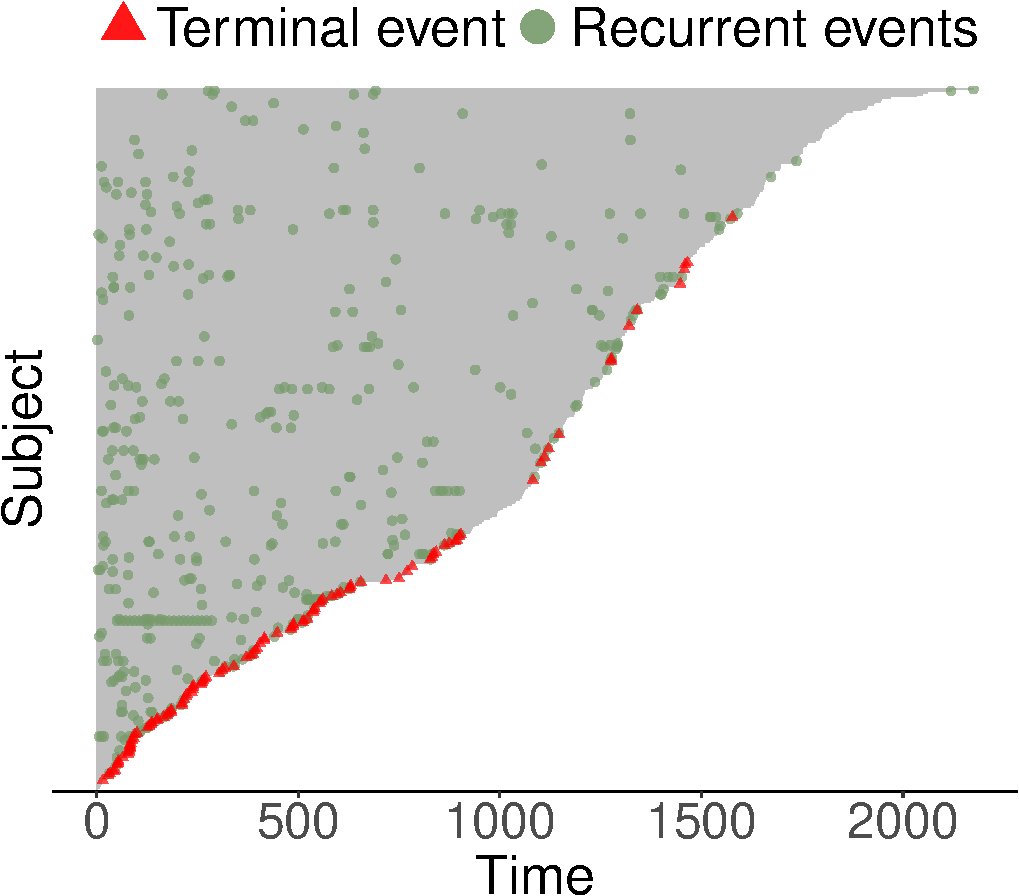
\includegraphics[scale = .25]{recur-figs/ep-1}
        \caption{No stratification}
    \end{minipage}\hfill
    \begin{minipage}{0.24\textwidth}
        \centering
        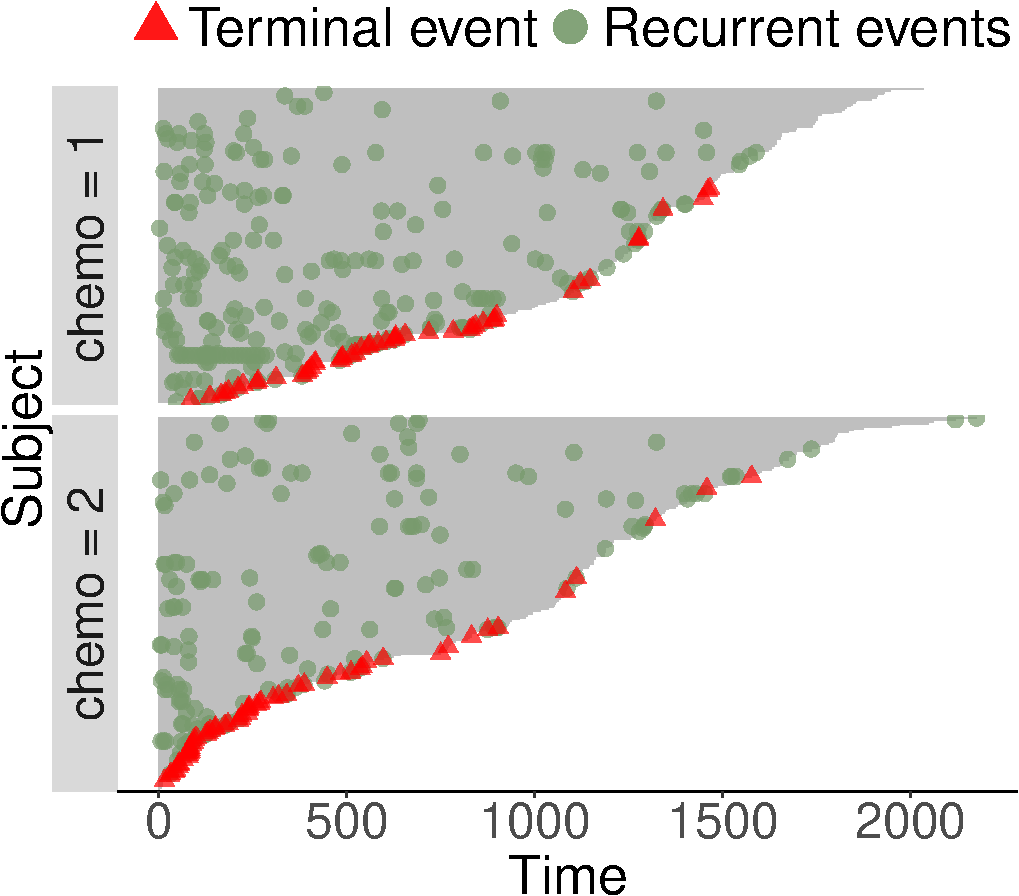
\includegraphics[scale = .25]{recur-figs/ep-2}
        \caption{Stratified by \texttt{chemo}.}
    \end{minipage}
\end{figure}


The mean cumulative function (MCF) is often the focus in a nonparametric
analysis of recurrent data. Let \(M_i(t)=\mathbb{E}\{N_i(t)\}\) denote
the MCF of \(N_i(t)\). The Nelson-Aalen estimator \citep{nelson2003siam}
are widely utilized in exploring the trend of recurrent event data.
\[\hat{M}(t) = \int_0^t \frac{dN(s)}{\delta(s)},\] where
\(dN(s)=\sum_{i=1}^k dN_i(s)\),
\(\delta(s) = \sum_{i=1}^k \delta_i(s)\), \(dN_i(s)\) and
\(\delta_i(s)\) is, respectively, the jump size and at-risk indicator of
process \(i\) at time \(s\). The MCF can be visualized by plotting the
\texttt{Recur} object with argument \texttt{MCF\ =\ TRUE} when the
\pkg{reReg} package is active. The \pkg{reReg} package also offers the
\texttt{plotMCF()} function for plotting MCF estimates to be stratified
by discrete variables. Alternatively, the \texttt{mcf()} function from
the \pkg{reda} package provides a more sophisticated approach to plot
MCFs. Some of the unique features the \texttt{mcf()} has include the
different variance estimations, confidence interval constructions, and
predictions. The following example uses the \texttt{mcf()} function to
visualize MCF estimates stratified by whether the patients receive
chemotherapy. The \texttt{plot()} method, as well as the
\texttt{plotEvents()} function, return a \texttt{ggplot2} object
\citep{hadley2016ggplot2} so that users may further customize the plot
easily.

\begin{Shaded}
\begin{Highlighting}[]
\NormalTok{re_mcf <-}\StringTok{ }\KeywordTok{mcf}\NormalTok{(fn, }\DataTypeTok{data =} \NormalTok{df0)}
\KeywordTok{plot}\NormalTok{(re_mcf, }\DataTypeTok{conf.int =} \OtherTok{TRUE}\NormalTok{, }\DataTypeTok{lty =} \DecValTok{1}\NormalTok{:}\DecValTok{2}\NormalTok{) +}
\StringTok{    }\NormalTok{ggplot2::}\KeywordTok{theme}\NormalTok{(}\DataTypeTok{legend.position =} \StringTok{"bottom"}\NormalTok{)}
\end{Highlighting}
\end{Shaded}

\begin{figure}[H]
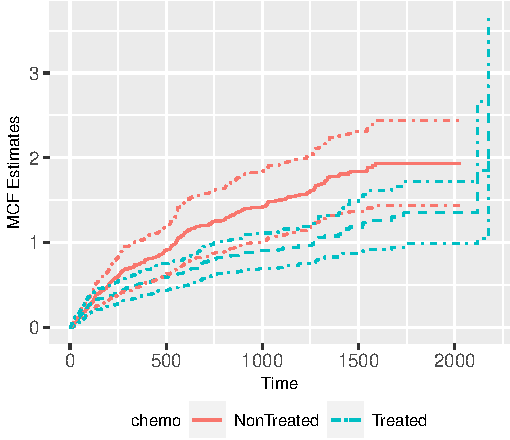
\includegraphics[scale = 1]{reda-mcf_files/figure-latex/plot-sampleMcf-1}
\end{figure}

Furthermore, the MCF difference between two groups can be tested with
the two-sample pseudo-score tests\\
\citep{cook1996biometrics} via \texttt{mcfDiff.test()} as follows:

\begin{Shaded}
\begin{Highlighting}[]
\KeywordTok{mcfDiff.test}\NormalTok{(re_mcf)}
\end{Highlighting}
\end{Shaded}

\begin{verbatim}
Two-Sample Pseudo-Score Tests:
                Statistic Variance  Chisq DF Pr(>Chisq)  
Constant Weight     47.49   416.71   5.41  1      0.020 *
Linear Weight       36.56   263.59   5.07  1      0.024 *
---
Signif. codes:  
0 '***' 0.001 '**' 0.01 '*' 0.05 '.' 0.1 ' ' 1

Variance Estimator: robust 
\end{verbatim}

Both the constant weighted and the linear weighted tests indicate the
MCF estimates are statistically different at a significance level of
0.05.


The \texttt{reReg()} function from the \pkg{reReg} package provides
methods to fit semiparametric regression models to recurrent event data.
A general joint model for the rate function of the recurrent event
process and the hazard function of the failure time can be formulated as
follow: \vspace*{-.5cm}

\begin{equation}
\lambda(t) = Z \lambda_0(te^{X^\top\alpha})e^{X^\top\beta};
h(t) = Z h_0(te^{X^\top\eta})e^{X^\top\theta},
\label{general}
\end{equation}

\vspace*{-.1cm}

where \(Z\) is a latent shared frailty variable to account for
association between the two types of outcomes, \(\lambda_0(\cdot)\) is
the baseline rate function, \(h_0(\cdot)\) is the baseline hazard
function, and the regression coefficients \((\alpha, \eta)\) and
\((\beta, \theta)\) correspond to the shape and size parameters of the
rate function and hazard function, respectively. In contrast to many
shared-frailty models that require a parametric assumption, following
the idea of \citet{wang2001analyzing}, the \texttt{reReg()} function
implements semiparametric estimation procedures that do not require the
knowledge about the frailty distribution. As a result, the dependence
between recurrent events and failure event is left unspecified and the
proposed implementations accommodate informative censoring.

Model \eqref{general} includes several popular semiparametric models as
special cases, which can be specified via the \texttt{method} argument
with the rate function and hazard function separated by
``\texttt{\textbar{}}''. For examples, the joint Cox model of
\citet{huang2004joint} is a special case of \eqref{general} when
\(\alpha = \eta = 0\) and can be called by
\texttt{method\ =\ "cox\textbar{}cox"}; the joint accelerated mean model
of \citet{xu2017joint} is a special case when \(\alpha = \beta\) and
\(\eta = \theta\) and can be called by
\texttt{method\ =\ "am\textbar{}am"}. Treating the terminal event as
nuisances (\(\eta = \theta = 0\)), \eqref{general} reduces to the
generalized scale-change model of \citet{xu2019generalized}, called by
\texttt{method\ =\ "sc\textbar{}."}. Moreover, users can mix the models
depending on the application. For example,
\texttt{method\ =\ "cox\textbar{}ar"} postulate a Cox proportional model
for the recurrent event rate function and an accelerated rate model for
the terminal event hazard function (\(\alpha = \theta = 0\) in
\eqref{general}). For inference, the asymptotic variance is estimated
from an efficient resampling-based sandwich estimator motivated by
\citet{zeng2008efficient}. The resampling approach is faster than the
conventional bootstrap as it only requires evaluating perturbed
estimating equations rather than solving them. The following code fits
the joint Cox model with 200 (default) resampling replicates:

\begin{Shaded}
\begin{Highlighting}[]
\KeywordTok{system.time}\NormalTok{(fit <-}\StringTok{ }\KeywordTok{reReg}\NormalTok{(fn, df0, }\DataTypeTok{method =} \StringTok{"cox|cox"}\NormalTok{))}
\end{Highlighting}
\end{Shaded}

\begin{verbatim}
   user  system elapsed 
  1.884   0.016   1.903 
\end{verbatim}

The \texttt{summary()} method prints the results of the model fits:

\begin{Shaded}
\begin{Highlighting}[]
\KeywordTok{summary}\NormalTok{(fit)}
\end{Highlighting}
\end{Shaded}

\begin{verbatim}
Call: 
reReg(formula = fn, data = df0, method = "cox|cox")

Recurrent event process:
             Estimate StdErr z.value p.value
chemoTreated   -0.189  0.244  -0.778   0.437

Terminal event:
             Estimate StdErr z.value p.value  
chemoTreated    0.519  0.286   1.815    0.07 .
\end{verbatim}

After a model is fitted, the baseline rate function and hazard function
can be visualized by plotting the \texttt{reReg()} object. See
\url{wenjie-stat.me/reda/} and \url{www.sychiou.com/reReg/} for the full
package documents.


\renewcommand{\bibsection}{\section*{Reference}}
\setlength{\bibhang}{0pt}
\setlength{\bibsep}{0.4em}
\bibliographystyle{asa}
\bibliography{ref}

\medskip

\noindent
\begin{minipage}[b]{1.2in}
\begin{flushleft}
\roundpic[xshift=0cm, yshift=-.4cm]{2.8cm}{4cm}{WenjieWang}
\end{flushleft}
\end{minipage}
\hspace{0.2cm}
\begin{minipage}[b]{2.4in}
\begin{flushright}
  \emph{Wenjie Wang}\\
  Research Scientist\\
  Machine Learning, Artificial Intelligence, and Connected Care\\
  Advanced Analytics and Data Sciences\\
  Eli Lilly and Company\\
  Email: \email{wang\_wenjie@lilly.com}
\end{flushright}
\end{minipage}
\newline\newline
\begin{minipage}[b]{1.2in}
\begin{flushleft}
\roundpic[xshift=0cm, yshift=-.5cm]{2.8cm}{2.8cm}{Chiou}\\
\end{flushleft}
\end{minipage}
\hspace{0.2cm}
\begin{minipage}[b]{2.4in}
\begin{flushright}
  \emph{Sy Han Chiou}\\
  Assistant Professor\\
  Department of Mathematical Sciences\\
  University of Texas at Dallas\\
  Email: \email{schiou@utdallas.edu}
\end{flushright}
\end{minipage}




\end{document}
